\section{Conditional KL Regularization in RL}

\begin{insight}
  In iterative algorithms, the target distribution helps separate intended gains from unintended side effects. For example, RL aims to maximize expected reward. With binary rewards, conditioning on $r(x,y)=1$ yields the training target $\pi_\theta^+$, which remains unchanged under the ideal update in \hyperref[lem:reward-reweighting]{Theorem~\ref*{lem:reward-reweighting}}. Tracking how this target changes during training can therefore reveal side effects beyond the intended reward improvement.
\end{insight}

\subsection{Conditional Decomposition in RL}

A sequence-level binary reward naturally decomposes the probability distribution induced by the original model into two components, with the true conditional distribution serving as the target distribution. The policy entropy also decomposes into the binary entropy of correctness and an accuracy-weighted average of the true and false conditional entropies.

\begin{lemma}[Accuracy-weighted entropy decomposition]
\label{lem:rl-target-entropy}
For a prompt $x$ with deterministic binary rewards, write $\rho=\rho_\theta(x)\in(0,1)$ for the accuracy and suppress conditioning on $x$. Let $H(\pi_\theta^+)$ and $H(\pi_\theta^-)$ denote the true conditional and false conditional entropies, respectively. Then
\begin{equation}
 H(\pi_\theta)=h_{\mathrm b}(\rho)
    +\rho H(\pi_\theta^+)+(1-\rho)H(\pi_\theta^-),
 \label{eq:rl-entropy-decomposition}
\end{equation}
where $h_{\mathrm b}(\rho)=-\rho\log\rho-(1-\rho)\log(1-\rho)$.
If $H(\pi_\theta^+)<H(\pi_\theta^-)$, increasing accuracy while keeping both conditional distributions fixed will decrease their weighted average entropy.
\end{lemma}
\noindent\hyperref[app:rl-target-entropy]{Proof: Appendix~\ref*{app:rl-target-entropy}.}

Typically in practice, both conditional entropies are much larger than the binary entropy $h_{\mathrm b}(\rho)\le\log 2$, the total entropy is well approximated by their accuracy-weighted average. This conditional is supported in our experiments, see Figure~\ref{fig:kl-ckl-comparison}. Both conditional entropies are significantly larger than the binary entropy, while false conditional entropy is usually several times higher than true conditional entropy.

This property can, to some extent, account for the approximately linear relationship between entropy and accuracy observed in prior studies~\citep{cui_entropy_2025}. However, a mere shift in probability density is insufficient to explain the reductions in diversity and pass@k performance reported in other studies~\citep{yue_does_2025, tajwar_maximum_2026}. This accuracy-driven source of entropy reduction in RL need not reflect a loss of diversity among correct responses. The concern with diversity collapse is the degeneration of the target and conditional entropy.

% In RL, entropy is only compariable when models exhibit similar sample accuracy.

This conditional decomposition induced by RL also offers a new perspective on regularization. To prevent model collapse and preserve generalization, a common practice is to introduce a KL-divergence constraint that keeps the trained model from deviating excessively from the original model~\citep{schulman_trust_2017, schulman_proximal_2017, ouyang_training_2022}. However, directly constraining the KL divergence can also limit improvements in reward. Under the conditional decomposition of RL, what we truly need to control is the degradation of the target distribution. This observation motivates a Conditional KL (CKL) regularization scheme that directly constrains changes in the target distribution.

This CKL regularization admits a simple policy-gradient estimator:

\begin{insight}
The mean log probability-ratio between the current and reference models over positive samples captures the average probability gain on correct solutions. CKL then regularizes only the deviation of each positive sample from this average gain. This actually introduces a baseline into the KL penalty for positive samples, while imposing no constraint on negative samples.
\end{insight}

\begin{theorem}[Centered sequence-$k_1$ estimator for CKL]
\label{thm:ckl-estimator}
Fix a prompt $x$ and suppress its conditioning. Let $\pi_\theta$ be a differentiable positive policy and $\pi_{\mathrm{ref}}$ a fixed reference. Define
$K(\theta)=D_{\mathrm{KL}}(\pi_\theta^+\Vert\pi_{\mathrm{ref}}^+)$.
Draw $G$ independent responses $Y_i\sim\pi_{\theta_0}$, and let
$I^+=\{i:r(x,Y_i)=1\}$ and $N=|I^+|$. The empirical signal is
\begin{align}
  d_i=\log\frac{\pi_{\theta_0}(Y_i)}{\pi_{\mathrm{ref}}(Y_i)}
%  =\sum_t\log\frac{\pi_{\theta_0}(Y_{i,t}\mid x,Y_{i,<t})}{\pi_{\mathrm{ref}}(Y_{i,t}\mid x,Y_{i,<t})}
  ,\notag\qquad
  \widehat c_i =
 \begin{cases}
 d_i-\dfrac{1}{N}\sum_{j\in I^+}d_j,&i\in I^+,\ N\ge2,\\
 0,&\text{otherwise}.
 \end{cases}
 \label{eq:ckl-empirical-signal}
\end{align}
Writing $s_i=\left.\nabla_\theta\log\pi_\theta(Y_i)\right|_{\theta_0}$,
the estimator satisfies, for every $n$ with $\Pr(N=n)>0$,
\begin{equation}
 \mathbb E\!\left[\left.\frac1G\sum_{i=1}^G\widehat c_i s_i\,\right|N=n\right]
 =\frac{\max(n-1,0)}{G}\left.\nabla_\theta K(\theta)\right|_{\theta_0}.
 \label{eq:ckl-finite-gradient}
\end{equation}
Thus a detached reward $-\beta\widehat c_i$, with $\beta\ge0$, gives an expected policy-gradient contribution proportional to the negative conditional KL gradient.
\end{theorem}
\noindent\hyperref[app:ckl-estimator]{Proof: Appendix~\ref*{app:ckl-estimator}.}

\begin{figure}[htb]
  \centering
  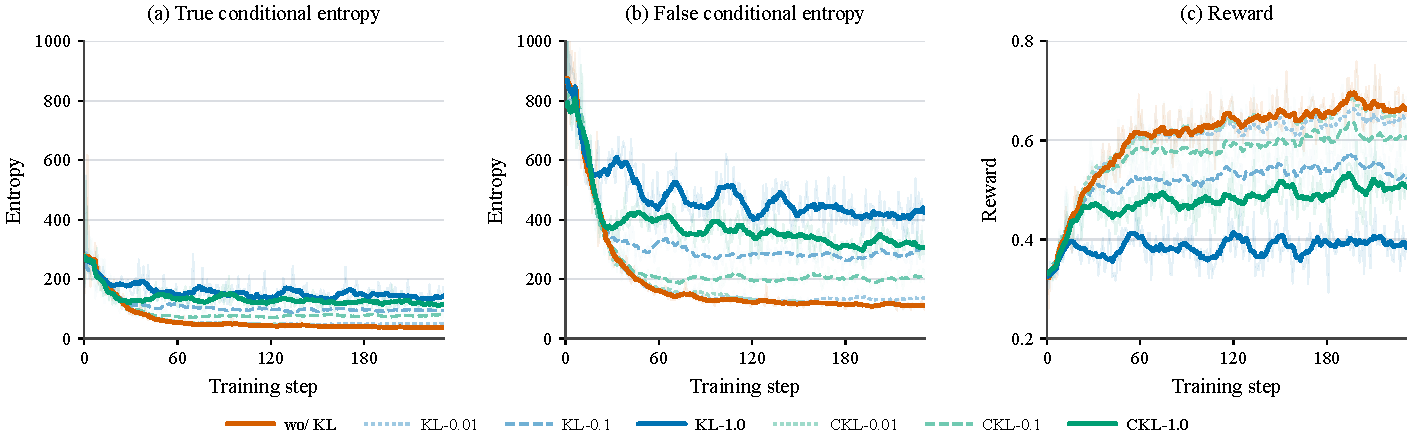
\includegraphics[width=\linewidth]{media/conditional_kl_comparison.pdf}
  \caption{The comparison of KL and Conditional KL (CKL) regularization in RL. We trained Qwen3-1.7B-Base~\citep{yang_qwen3_2025} on MATH~\citep{hendrycks_measuring_2021} dataset with GRPO~\citep{shao_deepseekmath_2024} algorithm and different KL penalities. Two conditional entropies are measured on the sequence level. We can see that strong KL control strength severely limits the reward increment in RL, while CKL regularization allows the model to obtain higher reward while maintaining the diversity of true samples.}
  \label{fig:kl-ckl-comparison}
\end{figure}

\begin{figure}[!htb]
  \centering
  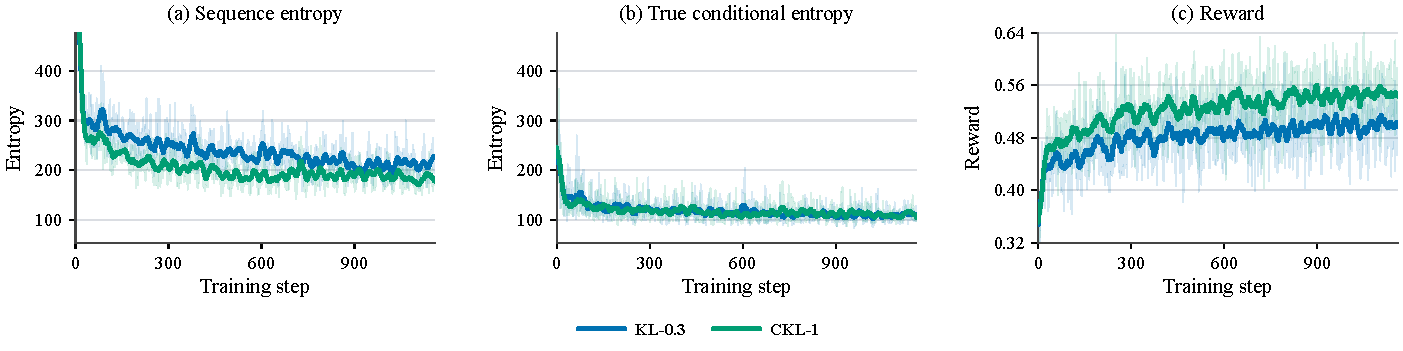
\includegraphics[width=\linewidth]{media/extended_conditional_kl_comparison.pdf}
  \caption{Extended experiments on KL and CKL regularization. These experiments follows the same setting as that in Figure~\ref{fig:kl-ckl-comparison}. We can see that CKL-1 and KL-0.3 exhibits similar regularization ability on conditional distribution, while CKL-1 constantly obtains higher accuracy. Its entropy will thus be slightly lower according to the accuracy-weighted decomposition.}
  \label{fig:ext-ckl-cmp}
\end{figure}

As shown in Figure~\ref{fig:kl-ckl-comparison}, we indeed observe that CKL effectively relaxes the constraint imposed by standard KL regularization on accuracy improvements while preserving the true conditional entropy. Although CKL cannot achieve completely lossless regularization due to cross-sequence interactions induced by model parameterization, it nevertheless demonstrates substantial practical value.

% We also evaluated these models on various test sets. As we can see in Figure~\ref{fig:passk-eval}, although on certain datasets such as Apex2025, the pass@k performance of the base model still surpasses the CKL regularized RL model, CKL still exhibit weaker collapse with higher accuracy compared with standard KL under the same control strength.

This advantage of CKL still holds for up to 20 training epochs, as shown in Figure~\ref{fig:ext-ckl-cmp}. We then evaluated these models on different math datasets, where CKL regularization did exhibit higher performance and generalizability over KL of similar strength, See Figure~\ref{fig:passk-eval}. More related results could be found in Section~\ref{app:rl-exps}.

\begin{figure}[!htb]
  \centering
  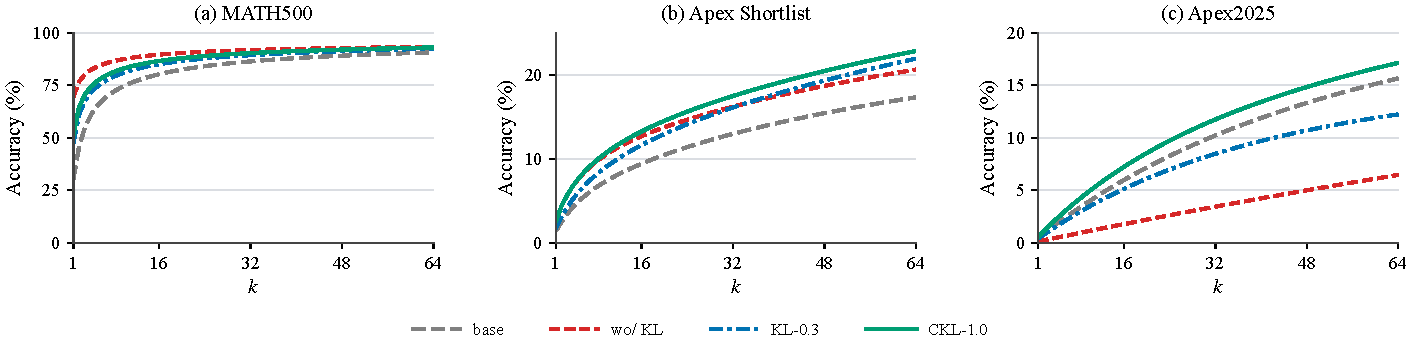
\includegraphics[width=\linewidth]{media/passk_comparison_epoch20.pdf}
  \caption{The comparison of pass@k performance on MATH500~\citep{lightman_lets_2023}, Apex Shortlist~\citep{balunovic_matharena_2025} and Apex2025~\citep{balunovic_matharena_2025}. Models are trained for 20 epochs on MATH dataset. We can see that models trained without KL has higher accuracy on datasets similar to the training set, while severe collapse occurs on harder datasets like Apex2025. CKL constantly achieves higher generalizability over KL regularization across these experiments.}
  \label{fig:passk-eval}
\end{figure}

% We characterize this term for one SGD update of a frozen-feature softmax readout at a fixed prefix $s$. Write $p_i=\pi_{W_0}(i\mid s)$ and $\varepsilon=\eta\|\phi(s)\|_2^2$. For a token subset $\mathcal S$ with equal expected advantage $A_i=a>0$, let $P_{\mathcal S}=\sum_{i\in\mathcal S}p_i$ and $q_i=p_i/P_{\mathcal S}$. With deterministic binary token rewards, $\mathcal S$ can be the success set, so $q$ is the true conditional target and $a=1-P_{\mathcal S}$.
%
% \begin{lemma}[First-order concentration under REINFORCE]
% \label{lem:rl-conditional-drift}
% Under this setup, a REINFORCE update gives
% \begin{equation}
%  \mathbb E[\Delta q_i]
%  =\varepsilon aP_{\mathcal S}q_i(q_i-M_2)+O(\varepsilon^2),
%  \qquad M_2=\sum_{j\in\mathcal S}q_j^2.
%  \label{eq:rl-conditional-drift}
% \end{equation}
% Tokens with $q_i>M_2$ gain conditional probability at first order. The first-order change in $H(q)$ is strictly negative unless $q$ is uniform, despite all tokens in $\mathcal S$ having equal expected advantage.
% \end{lemma}
% \noindent\hyperref[app:dynamics-reinforce]{Proof: Appendix~\ref*{app:dynamics-reinforce}, Lemma~\ref*{lem:dyn-reinforce}.}
%
% Related difficulties arise in classical RL, where policies can stall near suboptimal solutions. Log-barrier regularization helps maintain updates to low-probability actions and hence preserves the diversity~\citep{agarwal_theory_2020}. Under the same readout model, adding an inverse-probability correction with a constant signal cancels the first-order drift within $\mathcal S$.
%
% \begin{lemma}[First-order drift cancellation under normed-ls]
% \label{lem:rl-drift-cancellation}
% Under the same setup, adding the detached correction $a/(Vp_Y)$ to the sampled advantage in the REINFORCE loss gives normed-ls, where $V$ is the vocabulary size. This cancels the first-order expected drift of both the conditional distribution and its entropy:
% \begin{equation}
%  \mathbb E[\Delta q_i]=O(\varepsilon^2),
%  \qquad \mathbb E[\Delta H(q)]=O(\varepsilon^2).
%  \label{eq:rl-drift-cancellation}
% \end{equation}
% \end{lemma}
% \noindent\hyperref[app:dynamics-normed-ls]{Proof: Appendix~\ref*{app:dynamics-normed-ls}, Lemma~\ref*{lem:dyn-normed-ls}.}
%
% Note that this cancellation concerns the first-order mean drift; finite-step sampling noise can still change the conditional distribution and its entropy. The strict cancellation requires accurate estimation of per-token advantage, which is generally inaccessible in practice. So in the following experiments we used a simplified version of normed-ls method, using a constant to replace the advantage weight in the theoretical implementation. It already exhibits certain advantage over GRPO and MaxRL in experiments, while its performance equipped with a value model remains to be explored.

% TODO Experiments of normed-ls
